\section[An introduction to the red thread for this thesis]{An introduction to the red thread for this thesis}
\label{section_read_thread} 

A `red thread'~\footnotemark 
includes the core message of the thesis that's intended to keep the reader on track throughout the thesis. Here it's being used primarily to help me keep my work on message and enable me to discard topics and material that are too far removed from the red thread. This chapter is not written for publication, however some of the contents may be incorporated into the overall thesis.

\footnotetext{The term red thread is used in Scandinavian schools according to \href{https://writingcooperative.com/red-thread-and-other-writing-guidelines-4910b0d0d395}{‘Red Thread’ and Other Writing Guidelines}. An example of applying a red thread to a thesis is provided in \href{https://patthomson.net/2018/04/02/thesis-knowhow-how-the-contribution-can-create-coherence/}{thesis knowhow – “the contribution” can create coherence}. Tips on applying a red thread to improve a thesis are provided by a highly experienced PhD examiner in \href{https://threadreaderapp.com/thread/1192531751949737986.html}{Thread}. Others use a different colour, e.g. a \href{https://phdinahundredsteps.com/2015/05/26/spinning-the-golden-thread-that-can-sew-your-phd-together/}{a golden thread that can sew a PhD together}, and it may simply be a thread as follows: \href{https://www.thephdproofreaders.com/structure-a-phd/how-to-find-the-thread-that-runs-through-your-phd-thesis/}{How to find the thread that runs through your PhD thesis}.}

A key maxim for me is to: \emph{Always connect software engineering, mobile analytics, with the aim of improving reliability of mobile apps for end users.}



\clearpage
\section[Opening argument]{Opening Argument \\ \small{(Migrate to Conclusion and Abstract?)}}
If the mobile app and every supporting component in the system were reliable and complete we might not need or benefit from mobile analytics. Indeed they would be a distraction and wasteful. However, in the real-world every component be it software, service, system, person, or device has flaws and limitations. We are not omnipresent or omniscient. 
This raises three important questions that build from each other: 1) Could mobile analytics provide remote insights into a small yet vital subset of software quality? 2) Would this help development teams understand how their apps are performing in terms of their (un-) reliability? and 3) can that understanding help the developers address at least some of the underlying causes of the failures?

Pertinent information needs to flow from users' devices and reach the developers somehow in order for developers to understand the performance of their apps. 

Developer can plan for the future operations~\footnote{\emph{i.e.} the operations within the context of DevOps.} of the app in several ways, such as embedding code within an app to record events, context, and other data. They generally use an API to do so. Some of these sources of feedback are instigated by developers using logging and/or mobile analytics APIs, others are instigated by library and/or platform providers.
%
They can also plan various processes, ~\emph{e.g.} their release, bug investigation, and triage processes. Others may choose not to plan ahead; As many have observed, including the business guru Peter Drucker,~\emph{Not making a decision is a decision}, as summed up in Truth 31 in the book by~\cite{gunther2013truth_about_better_decision_making}.

Implicit feedback mechanisms provided by various forms of usage analytics (mobile analytics) can improve developers' awareness of how the software is being used and how it is behaving.  
The feedback mechanisms are used to identify probable issues in mobile apps where the development team then choose to address at least a subset of those issues with the aim of improving the quality-in-use~\citep{bevan1999_89_quality_in_use_meeting_user_needs_for_quality} of future releases of that app. 

\newthought{Scope}
Of the various forms of mobile analytics this research concentrates on \textbf{platform-level analytics} together with \textbf{crash and error analytics}. It applies these forms of analytics with a focus on improving \textbf{stability} of Android apps available in the Google Play Store.

%\akb{While it is right to focus on specific analytics, don't forget to explain the rationale for the ones you have chosen.} Agreed and will do when the content is migrated.

\newthought{Rationale}
The rationale for selecting these analytics include the vast scale and reach of the platform-level analytics in the largest app store globally where potentially billions of users rely on the quality of these apps and millions of developers have to trust and rely decisions that the Google Play store ecosystem applies for the apps they release in the app store. Furthermore the majority of Android apps include at least one analytics library that collects and reports crash and error analytics; both users and developers \emph{de-facto} trust these libraries are well behaved and can be depended on. Similarly users trust developers not to do net harm, a topic we cover shortly.

% For more reading on the nuances of the actions of doctors see:
% https://www.bmj.com/content/366/bmj.l4734/rapid-responses which includes a detailed clarification of "In illnesses one should keep two things in mind, to be useful rather than cause no harm".

\clearpage
\section[Research methodology]{Research methodology \\ \small{This may well become a new chapter.}}
The research is mainly empirical owing to the nature of usage analytics and the analytics tools which thrive on volume and realism therefore case studies provide the core of the research. Mixed methods were used to expand the research, for instance: by using static analysis into how developers use and maintain remote logging in the codebases of their Android apps, and qualitatively, by interviewing app developers on their use of mobile analytics. 

\newthought{Case Studies}
The case studies illustrate manifold facets of applying (and ignoring) mobile analytics across various contexts of engagement, across various types of app, and from several perspectives including the organizations who create the mobile analytics.

The case studies include examples where the researcher was:
\begin{enumerate}
    \itemsep0em
    \item embedded developer: an active participant integrated into the project team,
    \item coach: of an existing team of developers who applied the concepts,
    \item interviewer: of various development teams to learn of their practices and results,
    \item analyst/observer: performing static analysis of opensource code repositories.
\end{enumerate}

\clearpage
\section{Red Thread for the Case Studies}
\label{section-case-studies-red-thread}

Each case study needs to be formatted consistently so that the reader can find and compare any of them with any of the others, and establish patterns and connections as they're reading them, if indeed there are intentional patterns, orderings, and so on (beyond chronological).


TODO connect with ``Empirical research methods in software engineering"~\citep{Wohlin2003_empirical_research_methods_in_software_engineering}.

\subsection{Dimensions of the app case studies}
The following list is a proposed set of properties each case study would include:
{\small
\begin{itemize}
    \itemsep0em
    \item Role of the researcher?
    \item What are the focal points in this case study?
    \item Development practices of the project?
    \item Analytics sources: External, external + crash reporting, external + commercial internal, external, internal, and proprietary?
    \item Engagement level of the team?
    \item Privacy concerns?
    \item What opportunities did the case study present?
    \item What were the objectives (when I started the case study) compare and contrast with what actually happened? 
    \item What were the \textbf{F}indings and \textbf{I}nsights gleaned from each?
    \item What were the limitations of the tools that restricted the abilities to effect improvements? What were the limitations of the engineering practices that limited the improvements?
\end{itemize}
}

\begin{landscape} % Rotates the table into a landscape page in the generate PDF.
\definecolor{Gray}{gray}{0.9}
\begin{table}
    \setlength\extrarowheight{3pt} % provide a bit more vertical whitespace
    \captionsetup{size=footnotesize}
    \centering
    \tiny
    \tabcolsep=0.06cm
    %\rowcolors{1}{green}{pink}
    \begin{tabular}{lrrlllllllll}
        Label &Apps &Volumes &Role     &Focii       &Dev Practices &Analytics       &Objectives                   &Privacy &Opportunities &F.\&I.\footnote{Findings and Insights} \\
        \hline
        \rowcolor{Gray}
        Catrobat &2  &70.9K  &Coach     &Crashlytics &Sophisticated &Crashlytics    &M.A. vs. Clean Code          &Strong       &Open          &Immediate improvements \\
                 &   &190K   &Observer  &Control     &\textit{ditto} &              &Control for above            &ditto        &Open          &N/A \\ 
        
        \rowcolor{Gray}
        C1       &1  &1M+   &Consultant &at Scale   &Laminar        &Many           &Stability, Ways of Working   &Known        &Large-scale   &Rich \\
        GTAF     &11 &1.1M  &Observer   &Priorities &Team+          &Various        &Accurate local language apps &Strong       &Distinct view &Their priorities \\
        
        \rowcolor{Gray}
        Kiwix    &1  &150K  &Embedded   &P-o-C      &Team+          &Android Vitals &Suppress crash rate          &V.Strong     &Open, \nth{1} case study &It works!\\
                 &1  &58.9K &Observer   &Control    &\textit{ditto} &\textit{ditto} &Control for above            &\textit{ditto} &\textit{ditto} &\textit{ditto} \\
        \rowcolor{Gray}
                 &16 &222K  &Observer   &Scaling    &\textit{ditto} &\textit{ditto} &Measure scaling              &\textit{ditto} &\textit{ditto} &\textit{ditto} \\
        LocalHalo &1 &1.1K  &Observer   &Startup    &Cross-platform &Sentry.io      &New business view            &Unknown   &React-Native app &\\
        \rowcolor{Gray}
        Moodspace &1 &19.2K &Observer   &Startup    &TBC            &Crashlytics    &New business view            &Unknown   &            &Feedback on M.A.\\
        Moonpig  &1  &138K  &Observer   &Firebase   &Clean Code     &Firebase       &Leading edge practices       &Known     &Firebase insights &Insightful \\ 
    
        \rowcolor{Gray}
        Big C's  &10\textsuperscript{1} &10\textsuperscript{7} &Observer &Multi-teams &N/A &N/A      &Large corporate         &Unknown   &Big picture &   \\
        Analytics tools &10\textsuperscript{6} &10\textsuperscript{9} &Various &Trustworthiness &Various &Various &Improve the tools &Commercial &Bleeding edge &Flaws in tools \&services \\
    \end{tabular}
    \caption{Overview of App Case Studies}
    \label{tab:overview_of_app_case_studies}
\end{table}
\end{landscape}
%%%% Notes on compressing tables
% https://tex.stackexchange.com/questions/10766/how-to-make-really-wide-tables-narrower
% https://stackoverflow.com/questions/2563498/making-latex-tables-smaller
% https://en.wikibooks.org/wiki/LaTeX/Tables#Resize_tables 
% Smaller text finally worked after applying the tips from https://tex.stackexchange.com/a/56011/88466
% Row colors https://texblog.org/2011/04/19/highlight-table-rowscolumns-with-color/
% Rotate table https://tex.stackexchange.com/questions/370393/how-to-rotate-the-large-table-and-caption/370394
% Add a footnote https://tex.stackexchange.com/a/66641/88466
% Improvements in the formatting of the generated table https://tex.stackexchange.com/a/327977/88466




\newthought{Joe's suggestions}
\textit{Note: these will be merged into the rest of the thesis, here as a reminder until that's done.}

Joe is an industrial colleague. He proposed each case study could be formatted as a mini-paper with an abstract per case study.
{\small
\begin{itemize}
    \itemsep0em
    \item Which of the research questions does it answer?
    \item What’s the context? Mobile app? Web? Reporting tools? Library?
    \item What’s the company? Org structure? Communication tools?
    \item What tools were used? MS App Center, Android Vitals, etc. Crashlytics, Testing Frameworks, Collaboration tools,
    \item Team structure?
    \item How many users?
    \item Do the devs have access to the tools? how integrated into the development practices?
    \item Future work for each case study.
\end{itemize}
}
There are some overlaps and similar topics between the suggested dimensions of each case study and Joe's proposed list. TODO These two lists need to be harmonised, non-essential topics may be pruned from the combined list.


\subsubsection{Revised set of Marian's comments from our call on \nth{1} Sept 2021}

\newthought{The map is vital.}

There new tables aim to provide a partial map for the examiners so they don't get lost or side-tracked. They also help to clarify the thinking and make the case studies more consistent and coherent.

\begin{enumerate}
    \item \ref{tab:case-studies-research-perspective} \nameref{tab:case-studies-research-perspective}
    \item \ref{tab:case-studies-their-characteristics} \nameref{tab:case-studies-their-characteristics}
    \item \ref{tab:case-studies-findings-and-results} \nameref{tab:case-studies-findings-and-results}
\end{enumerate}

Notes: The previous table \ref{tab:overview_of_app_case_studies} \nameref{tab:overview_of_app_case_studies} may eventually be retired and removed from this red-thread. Another table, on the analytics tools, is also worth me creating.

Ideally a drawn map would complement these tables.

\newthought{Demonstrate competence as a researcher}

You need to be more precise in how you report the methodology, e.g., the case studies actually use mixed methods (not just the expansion). A methodology combines reasoning with the method. You need to convey rigour within the constraints of access to case studies.

At some point, you need a 'map' of the case studies:  these need to include the: case, methods, purpose...  This should give the reader an overview of what each contributes and where they overlap.

\newthought{Explain the challenges of anyone being permitted by teams to access their sensitive data, the opportunistic access and rigour applied in the case studies.}

Maximise my ability to make systematic use of what was pragmatically available: Opportunistic access, then I worked systematically and rigorously. Demonstrating the demands of rigour is vital. Explicit reporting of what I had and the efforts I made to handle the data systematically and be vigilant for bias. This helps avoid the case studies being considered as anecdotal. Amplify with the dialogues I had as part of the teams.

Start with what data did I collect and how I collected it. The case studies with similar sources of data can be compared which multiply the contribution.

Aim to explain what are the issues that arose in each case study?
A clear rationale needs to be provided. 

It's wise for the thesis to demonstrate there's a really clear audit trail and justification for the conclusions.

\begin{itemize}
    \item Characterise the case studies.
    \item Make explicit what data was collected and for what purpose. 
    \item Separate insights into a separate table. 
\end{itemize}

Quality of reporting of the empirical work is key

\newthought{Be Orthogonal and separate concerns}

Separate the reporting from the discussion.

\newthought{Next call with Marian} starts at 10:15 on Friday 10th Sept.

\begin{table}
    \centering
    \tabcolsep=0.06cm
    \tiny
    \begin{tabular}{lllll}\toprule
    Case Study                 & Role of Researcher &  Primary Method   & Opportunities & Purpose \\
    \midrule
    Kiwix                      & Embedded           & Action research   & & The experiment \\ 
    \textit{-"-} WikiMed (EN)  & Observer           & & Control for the above app & The control  \\
    \textit{-"-}               & Observer           & & Evaluate scalability & \textit{pico} generalisation \\
    Catrobat                   & Coach              & Action research   & & Compare Mobile Analytics with Clean Code \\
     \textit{-"-}              & Observer           & & Establish baseline & The control  \\
    C1                         & Consultant         & Hybrid/Mixed & Large scale complex commercial & Mission-critical view \\
    GTAF                       & Interviewer        & & Add'l perspective & Provide an Asian context \\
    LocalHalo                  & Interviewer        & & Add'l technologies & Hybrid Programming and tools \\
    Moodspace                  & Interviewer        & & Small startup &Bootstrap view \\
    Moonpig                    & Interviewer        & & Leading edge view & Mature, innovative, vanguard dev. practices \\
    Analytics tool providers   & Various            & & `Behind the curtain' & Learn about the providers' perspectives \\
    \bottomrule
    \end{tabular}
    \caption{Case Studies: the research perspective}
    \label{tab:case-studies-research-perspective}
\end{table}


\begin{table}
    \centering
    \tabcolsep=0.06cm
    \footnotesize
    \begin{tabular}{lcrcll}\toprule
    Case Study               & Apps                 & Reach & Context & Mobile Analytics Tools\textsuperscript{*}  &Dev. practices  \\
    \midrule
    Kiwix                    &                    1 &  150K & Wikipedia, FOSS            & GPC with AV &          Team+ \\ 
     \textit{-"-}            &                    1 & 58.9K & \textit{-"-}   & GPC with AV & \textit{ditto} \\
     \textit{-"-}            &                   16 &  222K & \textit{-"-}   & GPC with AV & \textit{ditto} \\
    Catrobat                 &                    1 & 70.9K & Coding, FOSS            & Crashlytics &  Sophisticated \\
     \textit{-"-}            &                    1 &  190K & \textit{-"-}   & GPC with AV & \textit{ditto} \\
    C1                       &                    1 &  1M+  & Mission-critical &    Multiple &        Laminar \\
    GTAF                     &                   11 &  1.1M & Another app category             &     Various &          Team+ \\
    LocalHalo                &                    1 &  1.1K & Risky early startup &   Sentry.io & Cross-platform \\
    Moodspace                &                    1 & 19.2K & Medical    & Crashlytics &        Startup \\
    Moonpig                  &                    1 & 138K  & E-commerce &    Firebase &     Clean Code \\
    Analytics tool providers &10\textsuperscript{6} &10\textsuperscript{9} & No &  Several &        Various \\
    \bottomrule
    \end{tabular}
    \caption[Case Studies: their characteristics]{Case Studies: their characteristics \\ {\tiny * All the apps used GPC with AV; one of the tool providers \emph{is} GPC with AV}}
    \label{tab:case-studies-their-characteristics}
\end{table}


\begin{table}
    \centering
    \tabcolsep=0.06cm
    \footnotesize
    \begin{tabular}{lllll}\toprule
    Case Study  & Results & Findings    & Insights & \\
    \midrule
    Kiwix                    &     & & It works! & Visibility drove action \\ 
     \textit{-"-}            &     & & \textit{ditto} & \\
     \textit{-"-}            &     & & \textit{It scaled} & Lead dev. took ownership \\
    Catrobat                 &        & & Immediate improvements & Ongoing ownership is vital \\
     \textit{-"-}            &     & & & \\
    C1                       &   & & OKRs achieved & Rich, multi-faceted \\
    GTAF                     &  & & & Their priorities  \\
    LocalHalo                &  & & Sentry.io \\
    Moodspace                &  & & Feedback on M.A. \\
    Moonpig                  &  & & Insightful \\
    Analytics tool providers &  & & Flaws in tools \& services\\
    \bottomrule
    \end{tabular}
    \caption{Case Studies: findings and results}
    \label{tab:case-studies-findings-and-results}
\end{table}


\subsection{Classifications of Mobile Analytics tools}
The case studies also facilitated the study of various mobile analytics tools. A map of these tools and the case studies they were used in may help the reader (and the author). Here are suggested topics to consider for each of these tools.
\begin{itemize}
    \itemsep0em
    \item To consider: which projects was the tool used in/relevant to?
    \item What was the tool used for?
    \item What insights did we glean from using the tool?
    \item If anythings made the tool distinctive, what were those things and why are they distinctive in the context of developers using mobile analytics?
\end{itemize}

%\href{section-case-studies-red-thread}{\nameref{section-case-studies-red-thread}} includes a table of the role the researcher played in each case study together with other pertinent details.

The research includes several aspects seldom studied owing to the challenges of obtaining the case studies, for instance from behind the curtain in commercial projects with over a million users, and from sources again seldom visible to researchers \emph{i.e.} of mobile analytics for real-world mobile apps.



\clearpage
\section[Phases of a release]{Phases of a release\\ \small{(Possibly integrate into Introduction, or into Preparing the Ground (Ch3))}}

%%% Thanks to
% https://tex.stackexchange.com/questions/69550/how-can-i-add-a-subtitle-to-a-section-title
% If I want to get fancy then https://tex.stackexchange.com/questions/417429/how-to-make-subheadings 

\begin{figure}
    \centering
    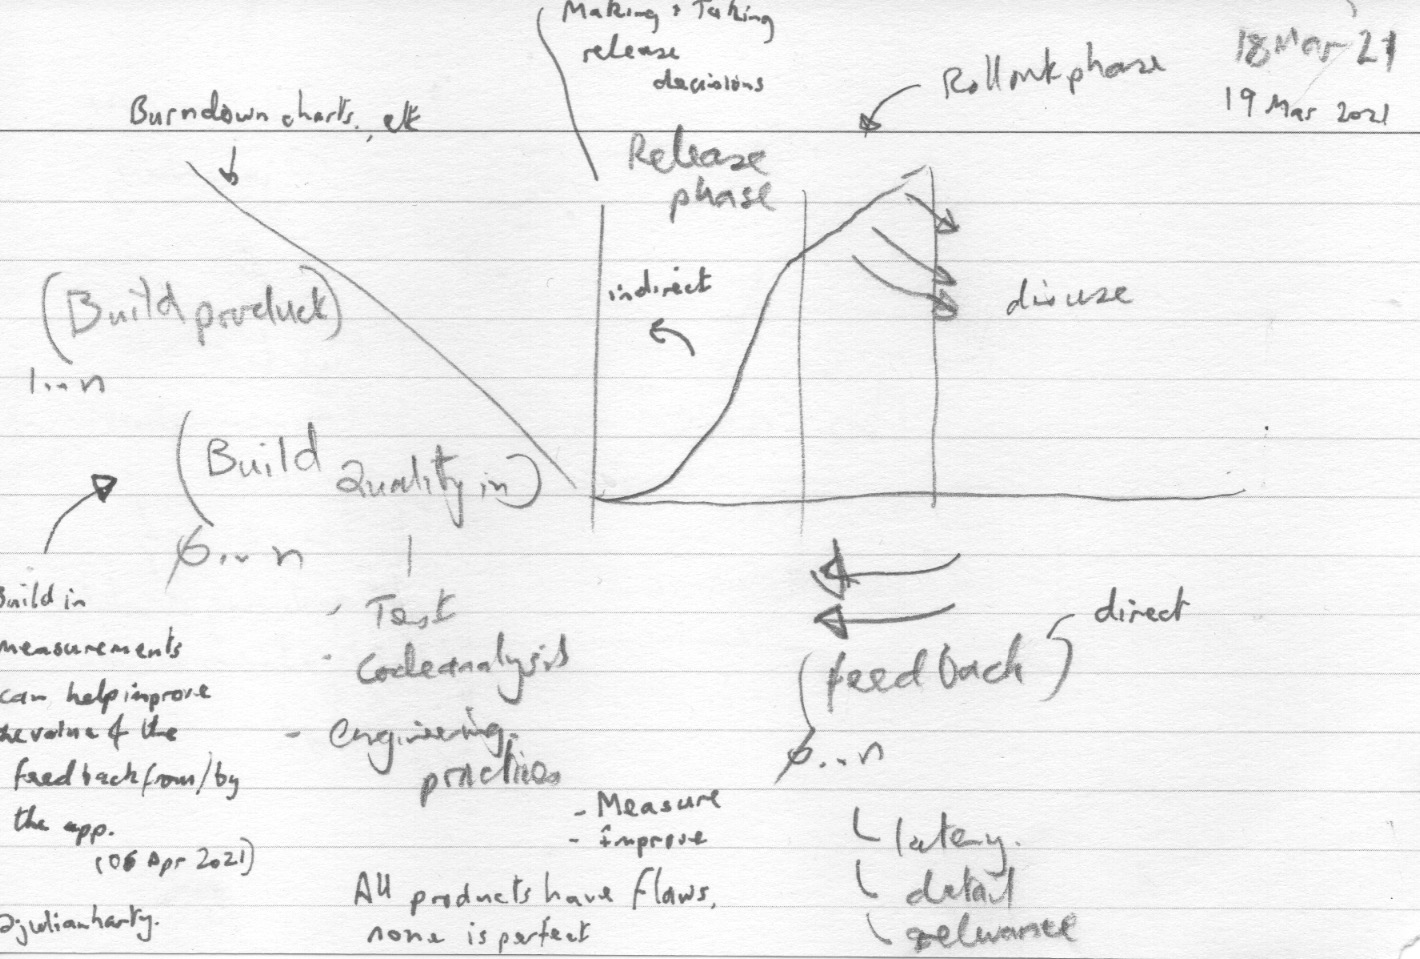
\includegraphics[width=15cm]{images/rough-sketches/Red-Thread-Rough-Sketch.jpeg}
    \caption{The lifecycle of a release and where mobile analytics provides feedback}
    \label{fig:red-thread-for-this-thesis}
\end{figure}

For any given release of a mobile app there are at least three material phases in order for the release to be used:
\begin{enumerate}
    \item Building the product: which may incorporate practices and tools intended to ship a `quality product'. Some teams also incorporate logging and reporting to help measure the behaviours of the app in use, post release.
    \item The Release: For some projects this may be as simple as uploading a new binary and making it fully available. For others they may incorporate decisions and mechanisms to make each release with the aim of de-risking any undesirable/adverse effects of the new release.
    \item Deployment: Deployment occurs when end users install and start using the release of the app. Both the app store and the end users affect when this occurs. App developers can try to hasten when users install the latest release through various mechanisms, for instance through implementing and mandating users upgrade their current release.
\end{enumerate}

Figure~\ref{fig:red-thread-for-this-thesis} illustrates these three phases together with some of the dynamics \emph{e.g.} of rollout and disuse of a release, and of feedback from whatever sources that the development teams can choose to pay attention to and apply. These phases are part of a longer lifespan of the release that includes an often long-term postdelivery period~\citep[pp 156-157]{evans2004_achieving_software_quality_through_teamwork} where users use the release until it is decommissioned or replaced with a subsequent release.

\begin{figure}
    \centering
    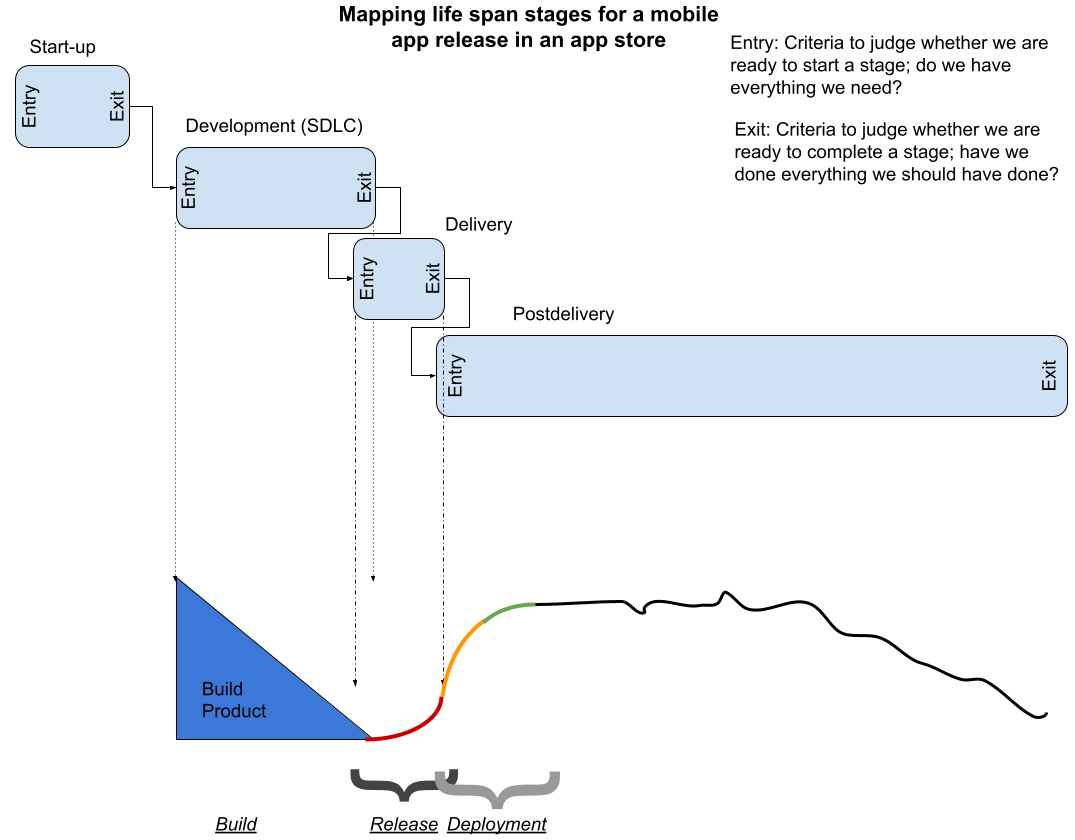
\includegraphics[width=16cm]{images/my/Mobile-app-life-span-stages.png}
    \caption{Mapping life span stages for a mobile app release in an app store}
    \label{fig:mobile-app-life-span-stages}
\end{figure}

Figure~\ref{fig:mobile-app-life-span-stages}~\footnote{Source of figure, Google Drive file: \href{https://docs.google.com/document/d/1d4B5l1tlpclHdKwY8W00qchiCV2YK5JjJP8TbkRHcjQ/edit}{Mobile app life span stages}.} compares a revised version of the `Life span stages' Figure in~\citep[p.155]{evans2004_achieving_software_quality_through_teamwork} mapped approximately to the three stages first illustrated in Figure~\ref{fig:red-thread-for-this-thesis}. Mobile app releases in an app store extend the Delivery which may also overlap either or both the development and the postdelivery life span stages. The overlap with the development stage is because the development is not complete until the app store accepts/approves the release (this may include pre-launch checks, automated testing, and so on depending on the app store). The overlap with deployment happens as releases are often released incrementally initially to a small percentage of the userbase - at least some of the users in that percentage will install the new release, until the percentage has been achieved. Meanwhile at least some of those users will use the app which will then mean the release is operational and may need operational support.


This research found that developers are able to materially improve the stability/reliability~\footnote{For Android Google used the term `stability' when they describe their Android Vitals service which is incorporated into Google Play Console. It effectively measures reliability for two specific types of failure: crashes and ANRs. An overview of Android Vitals is available online from various Google and Android sources including~\citep{android_vitals_overview_2019, android_vitals_best_practices}. HP also used the term `~\href{glossary-stability}{stability}' to measure crashes in mobile apps.}
%
of their mobile apps when they use the results of mobile analytics to assess the stability/reliability, identify groups of failures, triage the failures, and address the ones they decide to action. Where project teams stop paying attention to this process the failure rate increases of their new releases - the apps tend to entropy and failure.

Diligent developers and development teams can materially improve the stability/reliability of their apps through applying good coding, design and architecture patterns. Even these practices do not guarantee the releases will always be trouble-free. By paying ongoing attention to analytics during development, testing, and the rollout of releases flaws can be identified before the release reaches the majority of the userbase and teams can ameliorate the effects of many of the flaws.

\clearpage 

\section[Conceptual prerequisites]{Conceptual prerequisites\\ \small{(Possibly integrate into: Applying analytics to development practices?)}}
\begin{figure}
    \centering
    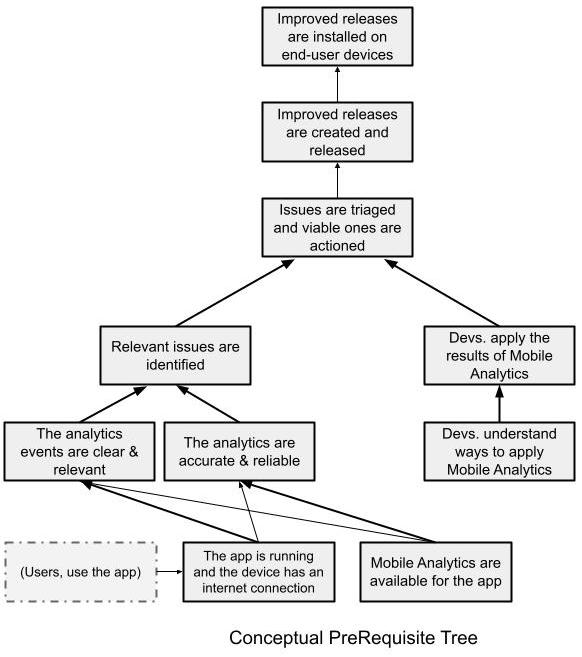
\includegraphics[width=12.5cm]{images/my/Conceptual_prereq_tree_Applying_Theory_of_Constraints_to_using_Mobile_Analytics_to_improve_Mobile_Apps.jpeg}
    \caption{Conceptual Prerequisites Tree: Using mobile analytics to improve mobile apps}
    \label{fig:using-toc-cpt-using-mobile-analytics-to-improve-mobile-apps}
\end{figure}


Figure~\ref{fig:using-toc-cpt-using-mobile-analytics-to-improve-mobile-apps}~\footnote{Source of figure, Google Drive file:  \href{https://docs.google.com/document/d/16PaSFRVzg1b2Nykly8qzaTAHtJqtEwgrK754wuek53M/edit}{2021 Applying Theory of Constraints to using Mobile Analytics to improve Mobile Apps}} illustrates a conceptual prerequisite tree \footnote{(applying Theory of Constraints, see~\citep{goldratt2017_necessary_but_not_sufficient, lepore1999_deming_and_goldratt, scheinkopf1999_thinking_for_a_change})}. 
%
The underpinnings in terms of being able to improve mobile apps are threefold: 
\begin{enumerate}
    \item Users need to use the app. The app's behaviours will include errors and failures.
    \item The app needs connectivity together with at least one form of mobile analytics.
    \item Developers need to understand the outputs of mobile analytics and address pertinent issues in future releases of the app.
\end{enumerate}

An expanded list of the prerequisites illustrated in Figuree~\ref{fig:using-toc-cpt-using-mobile-analytics-to-improve-mobile-apps} is as follows (roughly in descending order. Analytics data from previous releases is used to help improve \emph{future} releases.
{\small
\begin{enumerate}
    \itemsep0em
    \item Users use the app
    \item Improved releases are in-use on end-user devices
    \item Improved releases are installed on end-user devices
    \item Improved releases are created and released
    \item Analytics logging refined to capture relevant information
    \item Issues are triaged and viable ones actioned
    \item Devs have adequate, timely access to mobile analytics outputs
    \item Devs apply the results of mobile analytics outputs
    \item Devs understand ways to apply mobile analytics
    \item Relevant issues are identified and analysed
    \item The analytics service is accurate and reliable
    \item The analytics events are clear and relevant
    \item Volumes of data do not overwhelm system or devs
    \item The app is running and the device has an internet connection
    \item Mobile analytics are available for the app
\end{enumerate}
}


In addition to the previous set of prerequisites, the following are also highly desirable:
{\small
\begin{enumerate} [i]
    \itemsep0em
    \item Ecosystem is adequately and acceptably secure
    \item System is performant
    \item System is unbiased
    \item Internally and externally verifiable system and service
    \item Users have practical controls on the data processed
    \item Available data sufficiently representative to apply to the population
\end{enumerate}
}

\newthought{Addressing discovered issues}
Some issues can be ameliorated externally to the app, for instance though changes to servers that support API requests from apps, however many need changes to the app in order to be effective. 

If time-machines were available in software development developers might be able to go back in time and repair the current application on the user's mobile device. Conversely, a time-machine could enable users to return to the time and context when an event such as a failure occurred in order to help the developers understand contributory factors that led up to the failure and the aftermath. In 1999, time-machine computing was introduced as a way to help manage time in computing environments, for instance using a desktop environment - `TimeScape' - that supported time travelling on the computer, and time-casting to restore the context that surrounded the use of a given application~\citep{rekimoto1999_time_machine_computing}. In mobile analytics, breadcrumbs (event records)~\citep[p.683]{MacLean2015_pro_android_5_book} can be generated to help \emph{post-hoc} analysis of events that preceded a failure, and particularly crashes. 
%
For apps released as compiled binary files (the vast majority in iOS and Android app stores), improvements are generally made to a subsequent release than the one(s) where the failures have been occurring. And these subsequent releases need to be installed by the user population and used similarly in order to determine whether the improvements were worthwhile. Some users keep older releases and others stop using the app. 


% [4] Joorabchi, Mona Erfani, Ali Mesbah, and Philippe Kruchten. "Real challenges in mobile app development." Empirical Software Engineering and Measurement, 2013 ACM/IEEE International Symposium on 10 Oct. 2013: 15-24.

\clearpage
\section[Game Theory]{Game Theory\\ \small{(Possibly migrate to the Discussion chapter?)}}

\emph{Note: the current thesis doesn't have much on this topic. TBD whether to include it, it's certainly pertinent in my view.}

Many developers fail to address all the issues identified through use of mobile analytics and a key influence is their perceived ability to successfully address issues identified by the analytics. Furthermore, these issues are collectively only one of many demands for their time and attention. Human, organisational, and business factors all influence the extent mobile analytics is a) used and b) the results addressed. This research touches on both the mechanics of applying mobile analytics together with the `game' which are the higher-level human nature aspects which affect the application and the value of applying the mechanics. Figure~\ref{fig:the-mechanics-the-game} provides a simple illustration of the game and the mechanics.

\begin{figure}
    \centering
    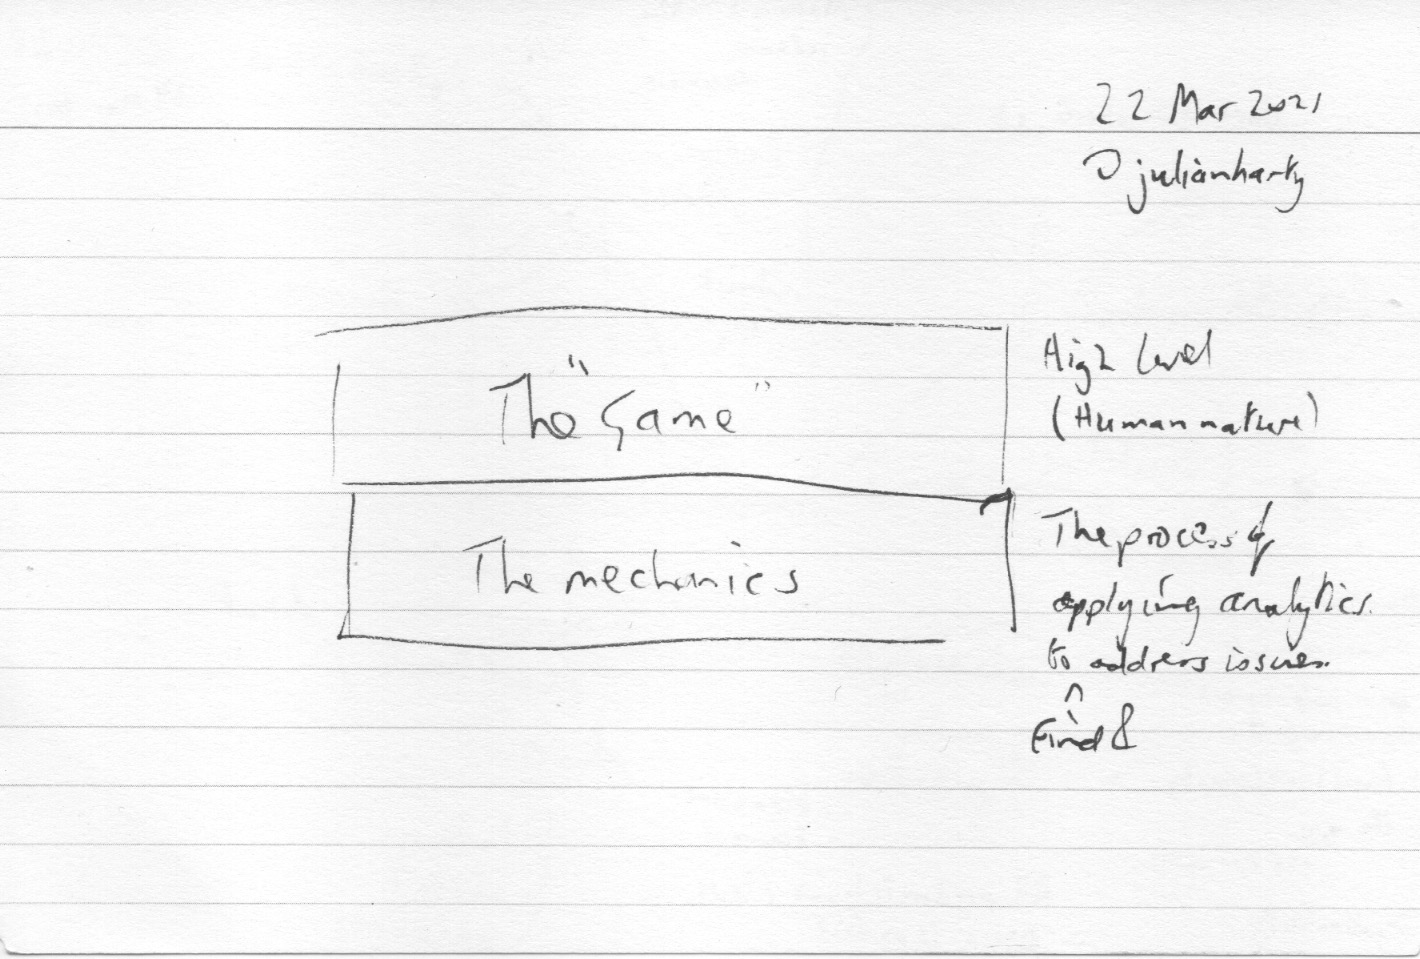
\includegraphics[width=15cm]{images/rough-sketches/The-Mechanics-The-Game.jpeg}
    \caption{The Mechanics and The Game of using Mobile Analytics}
    \label{fig:the-mechanics-the-game}
\end{figure}


\newthought{Living with risks} 
Risks include the risks of not using analytics and the risks of using analytics. Risk taking and risk aversion on the part of the developer, the team, the organisation, the app store organisation, and the end user come to play in the game.

Given the ongoing examples of misdeeds and corruptions in the application of data collected from user's activities and user's content - understanding and analysing the \href{glossary_data_dynamics}{[data] dynamics} of the information gathered, processed, and transferred in support of mobile analytics is also pertinent.

\newthought{Effort and rewards}
Significant data is available for minimal effort; paradoxically the lack of effort may lead to some developers underestimating the usefulness of using this data.

Development teams who choose to invest in analytics are able to reap better and more relevant results. Developers can choose to augment platform-level analytics with in-app analytics to augment or supersede aspects of what the platform provides.

\newthought{Risks and choices}
Developers can choose when they will pay attention to the analytics; they can also choose the extent they wish to integrate analytics into their apps. 

There are risks and responsibilities of the effects of collecting data and performing analysis on that data, practices outstrip legislation. It remains possible for sensitive findings to be discovered through the use of mobile analytics, nonetheless the ethical challenges are not unique to mobile analytics~\footnote{Arosha mentioned \href{https://www.orbit-rri.org/}{ORBIT-RRI} and their ~\href{https://www.journals.elsevier.com/journal-of-responsible-technology}{Journal of Responsible Technology}. There are various areas that overlap and potentially align in their concepts, I've not found much relevant concrete material yet, this footnote is a reminder (it is not intended to be part of my thesis.}.

\newthought{Freedom and responsibility}~\label{newthought-freedom-and-responsibility}
Developers often have more freedom in relation to how an app behaves than the users of their apps do. In practice the vast majority of Android apps in Google Play use and collect mobile analytics, the only material choice the users have is whether to use or not use a particular app. Sometimes the freedom is to \emph{not make a decision} (as mentioned earlier). Making a decision may have consequences. Not making a decision may have consequences. 

Who gets to choose may also be influenced by the larger organisation developers belong to. For example, in some large enterprises developers of an individual app may have to use prescribed mobile analytics rather than being able to make an independent [informed] choice.


\newthought{Minimise harm maximise value address material known issues}~\label{newthought-do-no-net-harm}
In the field of doctors there are discussions by \citealt{Schuenemann2011_guidelines2_0_do_no_net_harm} and \citealt{Sokolf6426_2013_first_do_no_harm_revisited} on \emph{do no net harm}. This has been eloquently adapted to \emph{``A competent and caring physician is one who never causes unintentional or unnecessary harm.", Stephen Ross Workman, MD}~\url{https://www.bmj.com/content/347/bmj.f6426/rr/671112}. Implicitly it could also apply to what users expect from the mobile apps they install and use. So, perhaps a the concept could be extended to the following maxim?: \emph{an app developer not only never causes unintentional or unnecessary harm, they also strive to address whatever harms do affect the users of their apps while also satisfying for other demands}~\footnote{In medicine there have been similar discussions on freedom and responsibility, and in particular on aftercare of what they publish~\citep{rennie1998_freedom_and_responsibility_in_medical_publication}.}.

\clearpage
\section[Practical aspects of using analytics]{Practical aspects of using analytics \\ \small{(Possibly migrate to the Conclusion? else the Discussion?)}}
Analytics providers have a major influence on the efficacy of the application of mobile analytics. There are limitations and flaws in the various tools this research has encountered regardless of their source (\emph{e.g.} in-house proprietary, opensource, free and paid-for commercial proprietary offerings). Nonetheless, flawed offerings are still able to be used to deliver improvements in the mobile apps. Specialised startups such as Iteratively aim to increase the coherence of embedded analytics (those embedded into the apps) while also increasing compliance. HP's AppPulse Mobile provided no-code analytics for mobile apps where their tools automatically instrumented the binary to add the analytics; several providers offered GUI interaction recording and `heatmaps' generated using aggregated recordings of touch screen interactions.

Those who applied the results of mobile analytics were able to increase the stability/reliability of their mobile apps. The amounts of improvements varied based on various factors such as:
\begin{itemize}
    \itemsep0em
    \item The starting point for the app.
    \item The amount of ongoing engagement of the development team.
    \item The choices of mobile analytics services and the use of proactive event recording using the related analytics libraries.
    \item The sources and causes of some of the issues being reported - some where far harder to diagnose than others, and several originated outside the actually codebase of the mobile app where it might be impractical to truly fix the source of the issue.
\end{itemize}

\noindent
\rule{\textwidth}{0.4pt}

\clearpage
\section{Where's my current focus?}
Right now, I'm migrating away from this chapter and working on establishing the first three sections in my Related Work chapter (Chapter 2).
